\begin{appendices}

%
% The first appendix must be "Self-appraisal".
%
\chapter{Self-appraisal}

\section{Critical self-evaluation}
Project strengths

Project limitations

Strengths of approach

Limitations of approach

\section{Personal reflection and lessons learned}
My progress individually

My lessons learned

\section{Legal, social, ethical and professional issues}
The following section covers the legal, social, ethical, and professional issues related to the project, and how we accounted for each.

\subsection{Legal issues}
Copyright

\subsection{Social issues}
Warzones?

\subsection{Ethical issues}
Privacy

\subsection{Professional issues}


%
% Any other appendices you wish to use should come after "Self-appraisal". You can have as many appendices as you like.
%
\chapter{External Material}\label{app:external_material}
This project uses material from various external source to aid in the implementation and testing of our solutions. All external material used is presented here.

\section{\code{Python} libraries}
The following is the full list of \code{Python} libraries used for the development of this project.
\begin{itemize}
    \item \code{Keras}
    \item \code{TensorFlow}
    \item \code{NumPy}
    \item \code{TensorFlow Datasets}
    \item \code{OpenCv--Python}
    \item \code{scikit--image}
    \item \code{scikit--learn}
    \item \code{matplotlib}
    \item \code{glob}
    \item \code{Pandas}
\end{itemize}

\section{NWPU-RESISC45 dataset}
The NWPU-RESISC45 dataset was accessed and loaded through the \code{TensorFlow Datasets} library. The dataset must be manually placed in the correct repository in the \code{TensorFlow Datasets} directory prior to using the data loader function. 

The dataset was downloaded from: \textcolor{blue}{https://1drv.ms/u/s!AmgKYzARBl5ca3HNaHIlzp\_IXjs}

\section{Set5 and Set14}
Set5 and Set14 are widely available online due to their widespread use. For this project, we used the public GitHub repository for the SelfExSR model as the source for the datasets. The repository was cloned and the appropriate LR and HR pairs were extracted.

The repository can be found here: \textcolor{blue}{https://github.com/jbhuang0604/SelfExSR}

\section{SRGAN implementation}
Whilst implementing SRGAN from scratch we used an online implementation~\cite{srganImplementation} as a reference point to aid us when encountering issues: \textcolor{blue}{https://pyimg.co/lgnrx}

\section{Pretrained classifiers}
In this project we aimed to improve loss by using a variety of pretrained image classifiers. Each of the pretrained classifiers is available as a part of the \code{Keras} library. The full list is as follows:
\begin{table}[ht]
    \centering
    \resizebox{\textwidth}{!}{
        \begin{tabular}{llllllll}
            \toprule
            \textbf{Model} & \textbf{Size (MB)} & \textbf{Top-1 Accuracy} & \textbf{Top-5 Accuracy} & \textbf{Parameters} & \textbf{Depth} & \textbf{ms/step (CPU)} & \textbf{ms/step (GPU)} \\
            \midrule
            Xception & 88 & 79.00\% & 94.50\% & 22.9M & 81 & 109.4 & 8.1 \\ 
            VGG16 & 528 & 71.30\% & 90.10\% & 138.4M & 16 & 69.5 & 4.2 \\ 
            VGG19 & 549 & 71.30\% & 90.00\% & 143.7M & 19 & 84.8 & 4.4 \\ 
            ResNet50 & 98 & 74.90\% & 92.10\% & 25.6M & 107 & 58.2 & 4.6 \\ 
            ResNet50V2 & 98 & 76.00\% & 93.00\% & 25.6M & 103 & 45.6 & 4.4 \\ 
            ResNet101 & 171 & 76.40\% & 92.80\% & 44.7M & 209 & 89.6 & 5.2 \\ 
            ResNet101V2 & 171 & 77.20\% & 93.80\% & 44.7M & 205 & 72.7 & 5.4 \\ 
            ResNet152 & 232 & 76.60\% & 93.10\% & 60.4M & 311 & 127.4 & 6.5 \\ 
            ResNet152V2 & 232 & 78.00\% & 94.20\% & 60.4M & 307 & 107.5 & 6.6 \\ 
            InceptionV3 & 92 & 77.90\% & 93.70\% & 23.9M & 189 & 42.2 & 6.9 \\ 
            InceptionResNetV2 & 215 & 80.30\% & 95.30\% & 55.9M & 449 & 130.2 & 10 \\ 
            MobileNet & 16 & 70.40\% & 89.50\% & 4.3M & 55 & 22.6 & 3.4 \\ 
            MobileNetV2 & 14 & 71.30\% & 90.10\% & 3.5M & 105 & 25.9 & 3.8 \\ 
            DenseNet121 & 33 & 75.00\% & 92.30\% & 8.1M & 242 & 77.1 & 5.4 \\ 
            DenseNet169 & 57 & 76.20\% & 93.20\% & 14.3M & 338 & 96.4 & 6.3 \\ 
            DenseNet201 & 80 & 77.30\% & 93.60\% & 20.2M & 402 & 127.2 & 6.7 \\ 
            NASNetMobile & 23 & 74.40\% & 91.90\% & 5.3M & 389 & 27 & 6.7 \\ 
            NASNetLarge & 343 & 82.50\% & 96.00\% & 88.9M & 533 & 344.5 & 20 \\ 
            EfficientNetB0 & 29 & 77.10\% & 93.30\% & 5.3M & 132 & 46 & 4.9 \\ 
            EfficientNetB1 & 31 & 79.10\% & 94.40\% & 7.9M & 186 & 60.2 & 5.6 \\ 
            EfficientNetB2 & 36 & 80.10\% & 94.90\% & 9.2M & 186 & 80.8 & 6.5 \\ 
            EfficientNetB3 & 48 & 81.60\% & 95.70\% & 12.3M & 210 & 140 & 8.8 \\ 
            EfficientNetB4 & 75 & 82.90\% & 96.40\% & 19.5M & 258 & 308.3 & 15.1 \\ 
            EfficientNetB5 & 118 & 83.60\% & 96.70\% & 30.6M & 312 & 579.2 & 25.3 \\ 
            EfficientNetB6 & 166 & 84.00\% & 96.80\% & 43.3M & 360 & 958.1 & 40.4 \\ 
            EfficientNetB7 & 256 & 84.30\% & 97.00\% & 66.7M & 438 & 1578.9 & 61.6 \\ 
            EfficientNetV2B0 & 29 & 78.70\% & 94.30\% & 7.2M & ~ & ~ & ~ \\ 
            EfficientNetV2B1 & 34 & 79.80\% & 95.00\% & 8.2M & ~ & ~ & ~ \\ 
            EfficientNetV2B2 & 42 & 80.50\% & 95.10\% & 10.2M & ~ & ~ & ~ \\ 
            EfficientNetV2B3 & 59 & 82.00\% & 95.80\% & 14.5M & ~ & ~ & ~ \\ 
            EfficientNetV2S & 88 & 83.90\% & 96.70\% & 21.6M & ~ & ~ & ~ \\ 
            EfficientNetV2M & 220 & 85.30\% & 97.40\% & 54.4M & ~ & ~ & ~ \\ 
            EfficientNetV2L & 479 & 85.70\% & 97.50\% & 119.0M & ~ & ~ & ~ \\ 
            ConvNeXtTiny & 109.42 & 81.30\% & ~ & 28.6M & ~ & ~ & ~ \\ 
            ConvNeXtSmall & 192.29 & 82.30\% & ~ & 50.2M & ~ & ~ & ~ \\ 
            ConvNeXtBase & 338.58 & 85.30\% & ~ & 88.5M & ~ & ~ & ~ \\ 
            ConvNeXtLarge & 755.07 & 86.30\% & ~ & 197.7M & ~ & ~ & ~ \\ 
            ConvNeXtXLarge & 1310 & 86.70\% & ~ & 350.1M & ~ & ~ & ~ \\
            \bottomrule
        \end{tabular}
    }
    \caption{The full list of pretrained image classifiers available from \code{Keras}, complete with accuracy metrics.}
\end{table}

\chapter{Additional results}
This appendix lists the full performance results for the first and second passes of each model, measured with SSIM and PSNR.\@
\section{SSIM}
\begin{table}[h!]
    \centering
    \begin{tabular}{llll}
        \toprule
        \textbf{} & \textbf{Test set} & \textbf{Set5} & \textbf{Set14} \\
        \midrule
        \textbf{SRResNet} & \textbf{0.923512511} & \textbf{0.764288652} & \textbf{0.656266853} \\ 
        \textbf{SRGAN-VGG22-A} & 0.905764824 & 0.651937458 & 0.567257665 \\ 
        \textbf{SRGAN-VGG22-B} & 0.899406253 & 0.583057506 & 0.513103986 \\ 
        \textbf{SRGAN-VGG54-A} & 0.885763096 & 0.581977762 & 0.543001687 \\ 
        \textbf{SRGAN-VGG54-B} & 0.887826756 & 0.668649288 & 0.60303856 \\ 
        \textbf{SRGAN-Xception-A} & 0.88827486 & 0.594680597 & 0.551749692 \\ 
        \textbf{SRGAN-Xception-B} & 0.893502931 & 0.672196794 & 0.601761352 \\ 
        \textbf{SRGAN-ResNet152V2-A} & 0.897174099 & 0.604043834 & 0.553452834 \\ 
        \textbf{SRGAN-ResNet152V2-B} & 0.891586191 & 0.661280537 & 0.602065958 \\ 
        \textbf{SRGAN-InceptionV3-A} & 0.895036106 & 0.652690864 & 0.593326379 \\ 
        \textbf{SRGAN-InceptionV3-B} & 0.897317878 & 0.686002073 & 0.616420747 \\ 
        \textbf{SRGAN-InceptionResNetV2-A} & 0.897677893 & 0.64776438 & 0.587032919 \\ 
        \textbf{SRGAN-InceptionResNetV2-B} & 0.901842292 & 0.682449324 & 0.610296856 \\ 
        \textbf{SRGAN-MobileNetV2-A} & 0.880168377 & 0.646061649 & 0.586623268 \\ 
        \textbf{SRGAN-MobileNetV2-B} & 0.892767837 & 0.692512978 & 0.616935856 \\ 
        \textbf{SRGAN-DenseNet201-A} & 0.906292091 & 0.68875187 & 0.625844913 \\ 
        \textbf{SRGAN-DenseNet201-B} & 0.904457413 & 0.697771048 & 0.629857361 \\ 
        \textbf{SRGAN-NASNetLarge-A} & 0.890887913 & 0.631735007 & 0.575758199 \\ 
        \textbf{SRGAN-NASNetLarge-B} & 0.892950461 & 0.663674025 & 0.596643366 \\ 
        \textbf{SRGAN-EfficientNetV2L-A} & 0.894187301 & 0.545100159 & 0.506600485 \\ 
        \textbf{SRGAN-EfficientNetV2L-B} & 0.895758924 & 0.574972219 & 0.526297118 \\
        \bottomrule
    \end{tabular}
    \caption{The full list of SSIM results for SRResNet and both training passes of each SRGAN variation.}
\end{table}
\clearpage
\section{PSNR}
\begin{table}[h!]
    \centering
    \begin{tabular}{llll}
        \toprule
        \textbf{} & \textbf{Test set} & \textbf{Set5} & \textbf{Set14} \\
        \midrule
        \textbf{SRResNet} & \textbf{24.01698267} & 22.92709729 & 21.64800947 \\ 
        \textbf{SRGAN-VGG22-A} & 23.49328972 & \textbf{23.20232616} & \textbf{21.86280371} \\ 
        \textbf{SRGAN-VGG22-B} & 23.04977341 & 21.53465502 & 20.83574047 \\ 
        \textbf{SRGAN-VGG54-A} & 22.60240965 & 21.15867685 & 21.08800741 \\ 
        \textbf{SRGAN-VGG54-B} & 22.84813356 & 22.17587848 & 21.75984152 \\ 
        \textbf{SRGAN-Xception-A} & 22.83258858 & 21.21166409 & 20.90811321 \\ 
        \textbf{SRGAN-Xception-B} & 23.12606804 & 21.28395406 & 21.00604196 \\ 
        \textbf{SRGAN-ResNet152V2-A} & 23.10085499 & 21.04849148 & 21.00699857 \\ 
        \textbf{SRGAN-ResNet152V2-B} & 22.90267499 & 22.09173107 & 21.8309256 \\ 
        \textbf{SRGAN-InceptionV3-A} & 23.17347567 & 21.44583352 & 21.25388063 \\ 
        \textbf{SRGAN-InceptionV3-B} & 23.27200493 & 21.52440082 & 21.29319431 \\ 
        \textbf{SRGAN-InceptionResNetV2-A} & 23.30451732 & 21.88277315 & 21.07909838 \\ 
        \textbf{SRGAN-InceptionResNetV2-B} & 23.39098294 & 22.24528009 & 21.6065458 \\ 
        \textbf{SRGAN-MobileNetV2-A} & 21.78452233 & 21.08368593 & 20.58121556 \\ 
        \textbf{SRGAN-MobileNetV2-B} & 22.41608497 & 20.61076707 & 20.38898798 \\ 
        \textbf{SRGAN-DenseNet201-A} & 23.58496348 & 21.23221522 & 21.67087999 \\ 
        \textbf{SRGAN-DenseNet201-B} & 23.46598423 & 21.62907 & 21.78881868 \\ 
        \textbf{SRGAN-NASNetLarge-A} & 23.05990787 & 20.82933654 & 20.6679965 \\ 
        \textbf{SRGAN-NASNetLarge-B} & 23.02686718 & 20.86077465 & 20.96187622 \\ 
        \textbf{SRGAN-EfficientNetV2L-A} & 22.34285427 & 18.34391675 & 19.30080662 \\ 
        \textbf{SRGAN-EfficientNetV2L-B} & 22.53702017 & 19.64714065 & 20.00809338 \\
        \bottomrule
    \end{tabular}
    \caption{The full list of PSNR results for SRResNet and both training passes of each SRGAN variation.}
\end{table}

\chapter{Visualisations}
The following appendix offers some useful image visualisations of datasets and solution outputs.

\section{Set5}
\begin{figure}[H]
    \centering
    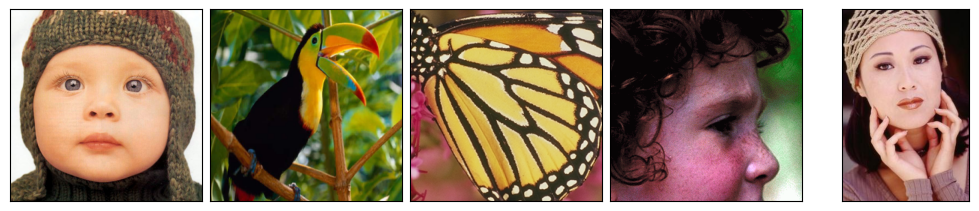
\includegraphics[width=\linewidth]{./assets/set5.png}
    \caption{The five images that make up the Set5 evaluation set.}
    \label{fig:model_comparison}
\end{figure}

\section{Set14}
\begin{figure}[H]
    \centering
    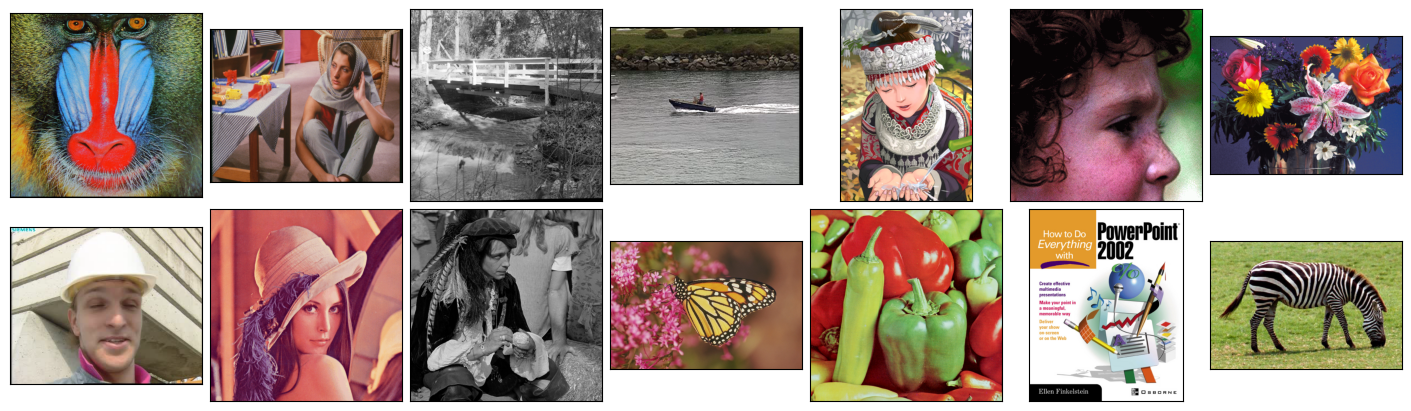
\includegraphics[width=\linewidth]{./assets/set14.png}
    \caption{The 14 images that make up the Set14 evaluation set.}
    \label{fig:model_comparison}
\end{figure}

\section{Model outputs}
\begin{figure}[H]
    \centering
    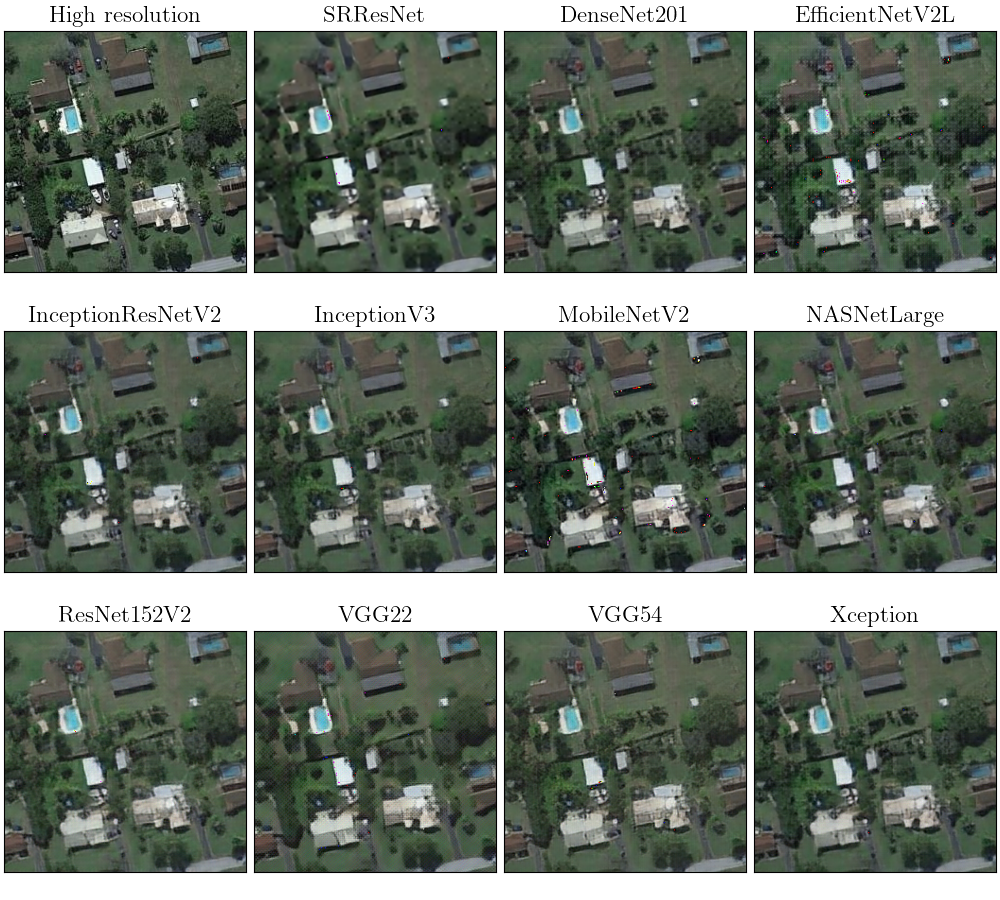
\includegraphics[width=\linewidth]{./assets/model_comparison.png}
    \caption{A comparison using a sample image from the NWPU-RESISC45 test set. The ground truth HR image, SRResNet, and SRGAN models with custom losses are shown.}
    \label{fig:model_comparison}
\end{figure}

\section{NWPU-RESISC45}
\begin{figure}[h]
    \centering
    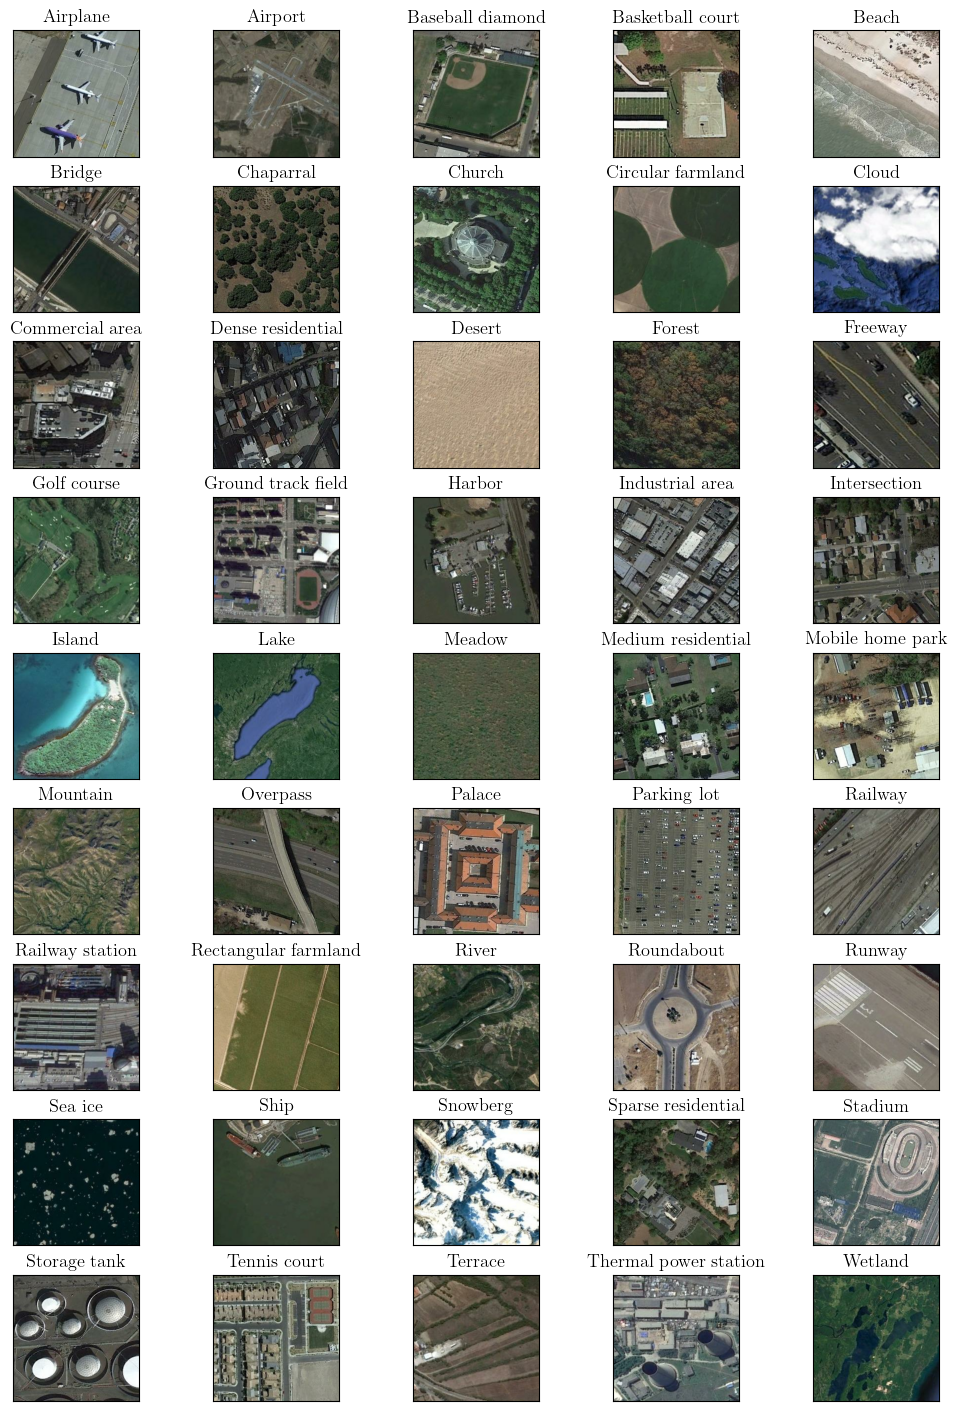
\includegraphics[width=\linewidth]{./assets/resisc45_all_classes.png}
    \caption{An example for each image class in the NWPU-RESISC45 dataset, taken from our test subset.}
\end{figure}

%
% Other appendices can be added here following the same pattern as above.
%



\end{appendices}
